\newif\ifshowsolutions
\showsolutionstrue
\documentclass{article}
\usepackage{listings}
\usepackage{amsmath}
%\usepackage{subfigure}
\usepackage{subfig}
\usepackage{amsthm}
\usepackage{amsmath}
\usepackage{amssymb}
\usepackage{graphicx}
\usepackage{mdwlist}
\usepackage[colorlinks=true]{hyperref}
\usepackage{geometry}
\usepackage{titlesec}
\geometry{margin=1in}
\geometry{headheight=2in}
\geometry{top=2in}
\usepackage{palatino}
\usepackage{mathrsfs}
\usepackage{fancyhdr}
\usepackage{paralist}
\usepackage{todonotes}
\setlength{\marginparwidth}{2.15cm}
\usepackage{tikz}
\usetikzlibrary{positioning,shapes,backgrounds}
\usepackage{float} % Place figures where you ACTUALLY want it
\usepackage{comment} % a hack to toggle sections
\usepackage{ifthen}
\usepackage{mdframed}
\usepackage{verbatim}
\usepackage[strings]{underscore}
\usepackage{listings}
\usepackage{bbm}
\rhead{}
\lhead{}

\renewcommand{\baselinestretch}{1.15}

% Shortcuts for commonly used operators
\newcommand{\E}{\mathbb{E}}
\newcommand{\Var}{\operatorname{Var}}
\newcommand{\Cov}{\operatorname{Cov}}
\newcommand{\Bias}{\operatorname{Bias}}
\DeclareMathOperator{\argmin}{arg\,min}
\DeclareMathOperator{\argmax}{arg\,max}

% do not number subsection and below
\setcounter{secnumdepth}{1}

% custom format subsection
\titleformat*{\subsection}{\large\bfseries}

% set up the \question shortcut
\newcounter{question}[section]
\newenvironment{question}[1][]
  {\refstepcounter{question}\par\addvspace{1em}\textbf{Question~\Alph{question}\!
    \ifthenelse{\equal{#1}{}}{}{ [#1 points]}: }}
    {\par\vspace{\baselineskip}}

\newcounter{subquestion}[question]
\newenvironment{subquestion}[1][]
  {\refstepcounter{subquestion}\par\medskip\textbf{\roman{subquestion}.\!
    \ifthenelse{\equal{#1}{}}{}{ [#1 points]:}} }
  {\par\addvspace{\baselineskip}}

\titlespacing\section{0pt}{12pt plus 2pt minus 2pt}{0pt plus 2pt minus 2pt}
\titlespacing\subsection{0pt}{12pt plus 4pt minus 2pt}{0pt plus 2pt minus 2pt}
\titlespacing\subsubsection{0pt}{12pt plus 4pt minus 2pt}{0pt plus 2pt minus 2pt}


\newenvironment{hint}[1][]
  {\begin{em}\textbf{Hint: }}{\end{em}}

\ifshowsolutions
  \newenvironment{solution}[1][]
    {\par\medskip \begin{mdframed}\textbf{Solution~\Alph{question}#1:} \begin{em}}
    {\end{em}\medskip\end{mdframed}\medskip}
  \newenvironment{subsolution}[1][]
    {\par\medskip \begin{mdframed}\textbf{Solution~\Alph{question}#1.\roman{subquestion}:} \begin{em}}
    {\end{em}\medskip\end{mdframed}\medskip}
\else
  \excludecomment{solution}
  \excludecomment{subsolution}
\fi

\newcommand{\boldline}[1]{\underline{\textbf{#1}}}

\chead{%
  {\vbox{%
      \vspace{2mm}
      \large
      Kelsi Riley \& Sakthi Vetrivel \hfill
      Caltech Earthquakes \hfill \\[1pt]
      Machine Learning \& Data Mining \hfill
      Caltech CS/CNS/EE 155 \hfill \\[1pt]
      Miniproject 3\hfill
      March $12^{th}$, 2018 \\
    }
  }
}

\begin{document}
\pagestyle{fancy}

% LaTeX is simple if you have a good template to work with! To use this document, simply fill in your text where we have indicated. To write mathematical notation in a fancy style, just write the notation inside enclosing $dollar signs$.

% For example:
% $y = x^2 + 2x + 1$

% For help with LaTeX, please feel free to see a TA!



\section{Introduction}
\medskip
\begin{itemize}

    \item \boldline{Group members} \\
    Kelsi Riley \\
    Sakthi Vetrivel
    
    \item \boldline{Team name} \\
    Caltech Earthquakes
    
    \item \boldline{Division of labour} \\
    % Insert text here.
    Kelsi implemented the HMM, and focused on improving it. She also did the preprocessing for the HMM, and the unsupervised algorithm. Sakthi implemented the RNN and worked on improvements for it, as well and the visualization and interpretation of the HMM.

\end{itemize}



\section{Pre-Processing}
\medskip
% Explain your data pre-processing choices, as well as why you chose these choices initially. What was your final pre-processing? How did you tokenize your words, and split up the data into separate sequences? What changed as you continued on your project? What did you try that didn't work? Also write about any analysis you did on the dataset to help you make these decisions.

\section{Unsupervised Learning}
\medskip
% This section should highlight your HMM. What packages did you use, if any? How did you choose the number of hidden states?



\section{Poetry Generation, Part 1: Hidden Markov Models}
\medskip
% Describe your algorithm for generating the 14-line sonnet. As an example, include at least one sonnet generated from your unsupervised trained HMM. You should comment on the quality of geneating poems in this naive manner. How accurate is the rhyme, rythym, and syllable count, compared to what a sonnet should be? Do your poems make any sense? Do they retain Shakespeare's original voice? How does training with different numbers of hidden states affect the poems generated (in a qualitative manner)? For the good qualities that you describe, also discuss how you think the HMM was able to capture these qualities.


\section{Poetry Generation, Part 2: Recurrent Neural Networks}
\medskip

% Explain in detail what model you implemented and using what packages. What parameters did you tune? Comment on the poems that your model produced. Does the LSTM successfully learn sentence structure and/or sonnet structure? How does an LSTM compare in poem quality to the HMM? How does it compare in runtime/amount of training data needed to the HMM? Include generated poems using temperatures of 1.5, 0.75, and 0.25 with the following initial 40-character seed: ``shall i compare thee to a summer\'��s day\n'', and comment on their differences.

\subsection{Initial Implementation}
For our preprocessing for the RNN, we decided to first break down the text file by line, and for each line we parsed, we made sure the line was not empty (not just an endline character) and removed any special characters from it. For example, we wanted to "Hello!" and "hello" to be processed as the same sequence of characters. We then finished each line with an endline character and added it to a accumulating string, which held the contents of the processed text file. After processing the input, we created dictionaries to convert each character found in the processed text to an integer, and a dictionary that converted integers to characters. We then generated a data set splitting this string into sequences of 40 consecutive characters, and converting the sequence of characters into a sequence of integers, and used the 41st character of the sequence as the y value, again, after converting it to an int.

We implemented a recurrent neural network using the Keras package for Python3. Using a sequential model, we had two dense LSTM layers of size 200, and one output layer. We calculated our loss using categorical cross-entropy loss, and 'adam' optimization. We also fine tuned our batch size, testing values of 32, 64, and 128. By observing the poems produced for these batch sized after 10 epochs of training, we settled on a batch size of 64. We also fine-tuned the size of the dense layers, trying sizes of 100, 150, and 200, as suggest in the project details, and settled of a size of 200. We then trained this model for 125 epochs, converging to a loss of 0.4146 from a loss of 3.45 after the first epoch. To improve our model, we also looked at more complex RNN, using two dropout layers between the dense layers, and fine tuned the dropout probability to eventually choose 0.4. Initially, the model was only trained for 20 epochs, but we found that the loss still hadn't converged so we continued training until the loss did not improve for 2 epochs. We used a window size of 40 as the instruction suggested, but later moved to smaller window size of 25 in our attempts to improve our model. 

To generate our poems, we used our seed sequence "Shall I compare thee to a summer's day?" and processed it, and for a sliding window of 40 characters, predicted the next letter in the sequence. Our model gives us an array of probabilities for the next character, given the previous 40 characters, so using this array of probabilities, we sample from the population of characters accordingly for a given diversity value. We also counted the number of newline characters that were predicted in the entire generation process, stopping after 14 newline characters, giving us 14 lines in the poem. 

Despite training for so many iterations, our LSTM did not successfully learn sentence structure or sonnet structure, as we see in the poems below, few of the words produced are real words. However, for the brief segments of the poems that contain real words, it seems to follow some loose sentence structure. For example: "i love you" and "of the braid". As a result, the poem quality seems fairly low, and this is a direct result of the character-based nature of the neural network resulting in jumbled English. Because there are so many more sequences of characters than sequences of words, the RNN takes more training data to train, but both sets of training data were still generated from the same text file. It took much longer to train the RNN than to train the HMM, again, because it starts from a lower level of understanding, since we are working with characters instead of words. 

\subsection{Poems}

\noindent
----- diversity: 1.5\\
----- Generating with seed: "  shall i compare thee to a summers day\\
"\\
  shall i compare thee to a summers day\\
weat kerp tellv in these i would to hath\\
my self iil iiddsu your thlltt my self brane ereed\\
but ceatt that weal i love you be teildde\\
and me altereasonse of the braid and lind\\
which treals mind eye is is a lawvereo\\
at tenmn lines bety paming iimeshsy\\
or at dolg pdr tiat weadddleditg tiink\\
eor shamls iampeut sp will he's shcd might\\
sevoy seep tidu thou 'liserpeas nor\\
j thak oyck tine suelt so lem so ku haln\\
  and nock i tas of fold cach or pattry\\
but be thy liate me thrnugh mights me sn botn\\
and in holaskeri hrln with the trwe doth green\\
and confoundane farth in thee tie live"\\


\noindent
----- diversity: 0.75\\
----- Generating with seed: "  shall i compare thee to a summers day\\
"\\
  shall i compare thee to a summers day\\
when that wilt nottncry that fell asd feidt\\
  that it 'bol gor moctatd i do dispilts\\
  and diary my self i'ck tren to the most\\
  but when your changent of this weil\\
byt sickt his tputatt mot i loow more eeee\\
to say toe borcmest whereup the bear\\
thy presclv ceauies ifart he lile artire\\
for whose winter's enoling on the rulp're\\
when sesimg a betteiry ocrure of thy deeds\\
therefo thy putlok dead trealed thou art\\
o what a worthsed wron delive no mane sehmnts\\
oo aly of these falsehe move's fresh ceserity\\
then the means me with vinter did stansed\\
and dotnt and in habkt and it gaults light"\\


\noindent
----- diversity: 0.25\\
----- Generating with seed: "  shall i compare thee to a summers day\\
"\\
  shall i compare thee to a summers day\\
aid uosthfr this wirte doth beauty stail\\
  thou mayst be thy oudsent'st a linit sade\\
  but when your count in these cannot chind\\
o carve norer mine him though mews the even\\
  but day doth daily draw my sorrows line\\
so thy freat gift woon be forgouingnl\\
for higheo of line ow well my heart deegines\\
so fotth the blow of with dupy steet selbit\\
  ald my hoade fyen siln liss lysbs'bd and were orisit\\
oatt reason haved the stard or thy sweet graces\\
beauteous all fellls tine world have erreemed\\
more that my self but was donf iis oun\\
gow many lambs kild and they acvodance seegng\\
and all the dead no nore drtbl dole"\\

\section{Additional Goals}
\medskip

% Explore methods of improving your poems or extending them. You do not need to attempt all of the tasks listed in the assignment for full marks on this section. If you have ideas for other improvements to the poetry generation not listed here, feel free to talk to a TA and work on it. The sky is the limit.

\subsection{Haikus}

We adapted our RNN to compose haikus. To do this, we created an file of haikus, where each line in a haiku in separated by a tab character, and each haiku is separated by a newline character. We also changed our window size from 40 characters to 15, since haikus are much smaller, and a 40 character seed would make up a significant portion of the poem. We continued to use dense layers of size 200. We then trained the RNN on this data set for about 100 epochs with a batch size of 64 (the batch size we found was effective for our sonnets). To generate our haikus, we used the same skeleton as the sonnets, just adjusting the window size. The results for the haikus were much more promising than the sonnets, which was surprising considering the training set was smaller. Here are some of our favorite haikus that were generated:\\

\begin{center}

light snowy breath	to read\\
old tombstones hot wind shadows\\
the roadrunner's beak\\

\bigskip

\noindent
furled umbrella\\
turns into a cane\\
chernobyl vells\\

\end{center}
 
Of course, many of the haikus we generated often contained just jumbled letters, and when they did contain words, they rarely made sense, much like the haikus above. However, the model was able to predict syllable count fairly accurately, as you can see the first haiku follows the 5-7-5 pattern, and the second haiku is close. Given more time, we would have liked to experiment with the Word2Vec package and worked to predict words that were similar to the previous words in the sequence.


\subsection{More Complex RNNs}

To improve our RNN, we decided to implement a more complex model. Instead of using two dense layers of size 200, we decided to include dropout layers as well to avoid overfitting.We also used a smaller window size of 25. Moreover, instead of predicting the character following a sequence, we trained the model to predict the character preceding the sequence. This was in preparation for us to generate rhyming poems.

Given the chance to do this again, we would have liked to also train with a validation set, and have stopped training when the validation loss stopped improving, instead of depending of the training loss. Here are the poems generated with this approach:

\medskip


\begin{flushleft}
----- Generating with end: ue by the grave and thee\\
----- Diversity: 0.25\\

\medskip
and in this cold complaining\\
she would have trained crie\\
and in his and he like again\\
my art thou art in me must roves to side thy state\\
and in your offences fived in your devory\\
of fathered bester and with dinkilling eye\\
that she more living so offence alove\\
in either kill of beauty tend\\
and with a concestion makes her wind\\
and with your shame to supretise is scapening on to love my love\\
that my after for my days dad make the mettle wit\\
against my valthough it should nor gistless\\
cinfounded in a mined eyes\\
the tongue by the grave and thee\\
\medskip
----- Diversity: 0.75\\
\medskip
but loves her painted hend\\
with whose what eyes now love to my\\
and that can men shall heavenly for see only most to shows and toney\\
to make the mudder's grace\\
for thy sweet to time's eyes to hast\\
but no so is my love to cay\\
and to the humbers at the spirit on thee\\
'didst thou the sefle but in his rain\\
to from the best this true for then the eye alone\\
even in my love com from that at the reason\\
to lives my sorrow nature had't teou poy\\
to fair thy loses she lacks and unneed the bound to make their sidness\\
fit and the trembling eyes\\
the tongue by the grave and thee\\
\medskip
----- Diversity: 1.5\\
\medskip
i should in cartle's dame\\
was fined in lidob giden kies\\
then boldness her beauteous i will\\
hinour to elmantinal condensmaking\\
with those and burd nor let\\
to prubify to leave th from it\\
when shalt thou my have be end\\
so do am state at living eye and heart it may be gone
lix\\
the other hours are so co civitate\\
the colous o'erds to hell for love and bift from this all treed\\
and when that gave to trespect thy state\\
but were the had taught the cloud or all apay\\
and in her hourffece baskys-are tongue by the grave and thee\\
\end{flushleft}

\subsection{Rhyming}

For our rhyming using the RNN, we used this implementation of the more complex RNN. Our first step was to generate a rhyming dictionary using the CMU dictionary and parsing each line of the sonnets. Using the CMU dictionary, we generated the pronunciations of each of the words in the Shakespearean texts, and compared the pronunciations of the ending of each of the words, so each word mapped to the pronunciation of its ending, and each pronunciation mapped to a list of words with that ending. 

Now to generate the rhyming poem, we find the endings of each line and generate the preceding characters based on the word. First, we find 7 random words in the sonnets, and make these the ends of lines 1, 2, 5, 6, 9, 10, and 13. Then, we use our rhyming dictionary to choose a word that rhymes with the line endings of the aforementioned lines and make these words the endings of lines 3, 4, 7, 8, 11, 12, and 14, such that we have a $ababcdcdefefgg$ rhyme scheme. 

Below is one of the poems generated through this process:\\
\\
Have women witagainst the cause but in the horn,\\
The sparm'dall wither yet love me all contented stair,\\
To beand croused could back their mildress' sky forlorn,\\
Effects and dischance andmore beauty of thyself all stair.\\
But his smokest love some is and now appear,\\
With that praise for living chance or thy burn,\\
Friendand for thee and steared berience more you peer,\\
Lively and confounds his artand heavenly one can spurn.\\
That true whan attening of her lind and horse,\\
Thas thoosebut if the would be maunt the heart,\\
Of all love's sout'st she dings with thy scarce,\\
Eyesand never was so watch the for both's transport.\\
\indent
To the priseand sily burupt make tears they sphere,\\
\indent
Thoutment on that gave darefrown from the dangerous year.\\

\section{Visualization and Interpretation}
\medskip

% Explain your interpretation of how a Hidden Markov Model learns patterns in Shakespeare's texts. You should briefly elaborate on the methods you used to analyze the model. In addition, for at least 5 hidden states give a list of the top 10 words that associate with this hidden state and state any common features among these groups. Furthermore, try to interpret and visualize the learned transitions between states. A possible suggestion is to draw a transition diagram of your Markov model and give descriptive names to the states. Feel free to be creative with your visualizations, but remember that accurately representing data is still your primary objective. Your figures, tables, and diagrams should contribute to a discussion about your model.

\subsection{Visualization of dataset}

\begin{figure}[H]
\centering
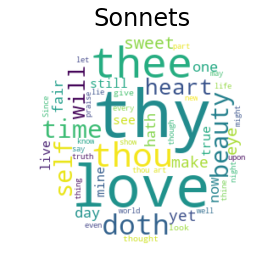
\includegraphics[width=90mm]{sonnets_wordcloud.png}
\end{figure}

\subsection{Visualization of the sparsities of A and O}

\begin{figure}[H]
\centering
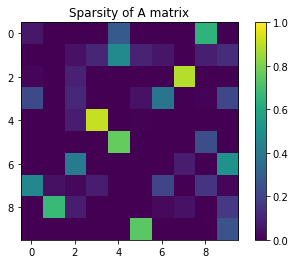
\includegraphics[width=90mm]{A_sparsity.png}
\end{figure}

\begin{figure}[H]
\centering
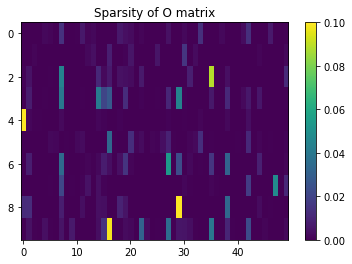
\includegraphics[width=90mm]{O_sparsity.png}
\end{figure}

% NEED TO REWORD THIS
Most elements of A and O are very close to 0. For the A matrix, this implies that at each state, there are only a few states to which the HMM will likely transition. For the O matrix, this implies that at each state, a few key observations are likely to be emitted. Usually, these correspond to frequently occurring words like "the", "and", "a", etc.

\end{document}
